\documentclass[12pt]{article}
\usepackage{amsmath}
\usepackage{graphicx}
\usepackage{float}
\begin{document}
\title{Electrical Engineering 141, Homework 6}
\date{March 1st, 2019}
\author{Michael Wu\\UID: 404751542}
\maketitle

\section*{Problem 1}

The open loop transfer function is the following.
\[\frac{K}{(s+1)^3}\]
This crosses the real axis when \(1+j\omega\) has a phase of \(\pm \frac{\pi}{3}\) or \(0\). This occurs
at \(\omega=0,\pm\sqrt{3}\). The magnitude of the open loop transfer function at these points are
\(K\) and \(-\frac{K}{8}\), respectively. The open loop transfer function has no poles in the right half
plane, so we should have no encirclements around \(-1\) in order to have a stable system. Since we know
that the value of the transfer function goes to zero as \(\omega\) goes to \(\infty\), we know that we
will have an encirclement if \(-\frac{K}{8}<-1\). On the positive side we also know we will have an
encirclement if \(K<-1\). Thus we want the following inequality to hold in order to have a stable system.
\[-1<K<8\]

\section*{Problem 2}

\paragraph{a)}

The Nyquist diagram is shown below.
\begin{figure}[H]
    \begin{center}
        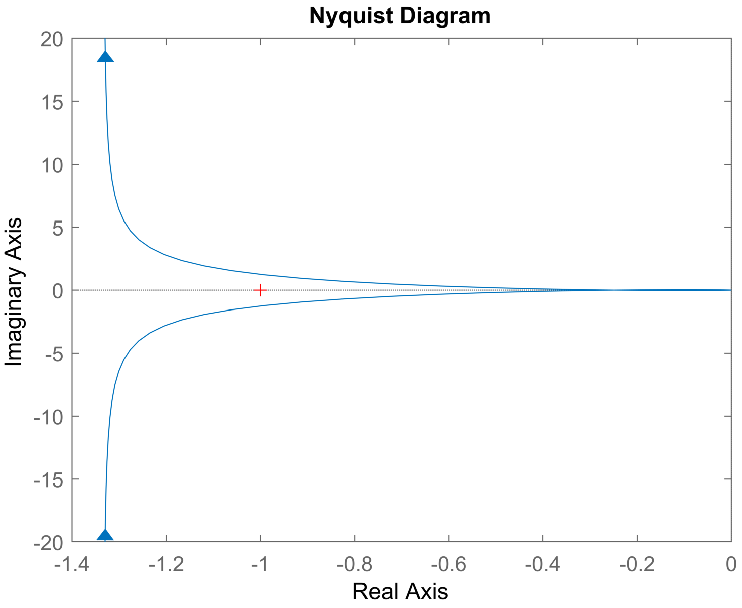
\includegraphics[width=3.5in]{problem2a.pdf}
    \end{center}
\end{figure}
The plot goes to infinity, and since we choose to not include the open loop pole at \(s=0\), we determine
that the loop connects on the right half plane. Thus the critical point is not contained within a loop, and
there are no unstable poles in the closed loop transfer function since the contour does not circle any open
loop poles.

\paragraph{b)}

The Nyquist plot crosses the real axis when \(j\omega(1+j\omega)(3+j\omega)\) is real. This can be rewritten
as the following expression.
\[-4\omega^2+j(3\omega-\omega^3)\]
This occurs when \(\omega=0,\pm \sqrt{3}\) and the corresponding magnitude of the transfer function is
\(K\infty\) and \(-\frac{K}{4}\). Thus we must have \(0<K<4\) in order to have a stable closed loop system.

\paragraph{c)}

If we have \(K>4\), then the critical point will have two clockwise loops around it. Then the Nyquist stability
criterion indicates that there will be two more closed loop poles than open loop poles in the right half plane.
Since we have zero open loop poles in the right half plane, this means there will be two closed loop poles in
the right half plane. If we have \(K<0\), then the critical point will have one clockwise loop around it. This corresponds
to one closed loop pole in the right half plane.

\paragraph{d)}

The root locus plot is shown below.
\begin{figure}[H]
    \begin{center}
        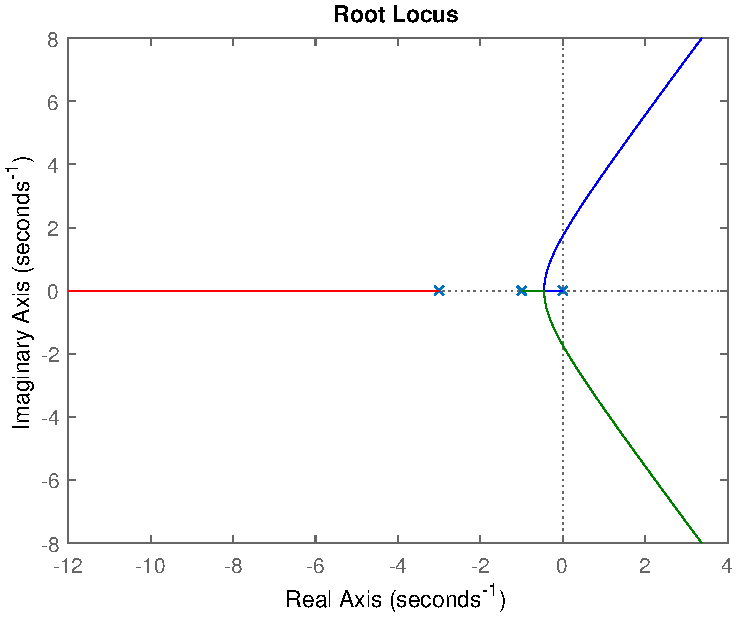
\includegraphics[width=3.5in]{problem2d.pdf}
    \end{center}
\end{figure}
This confirms that there will be two unstable poles as \(K\) increases above \(4\). Clearly the complementary
root locus plot indicates that there will be one unstable real pole if \(K\) is negative.

\section*{Problem 3}

\paragraph{a)}

\paragraph{b)}

\paragraph{c)}

\paragraph{d)}

\paragraph{e)}

\section*{Problem 4}

\paragraph{a)}

\paragraph{b)}

\paragraph{c)}

\paragraph{d)}

\section*{Problem 5}

\paragraph{a)}

\paragraph{b)}

\paragraph{c)}

\paragraph{d)}

\paragraph{e)}

\paragraph{f)}

\paragraph{g)}

\end{document}